% The classes of functions, nested, with one example each.
%
%   figures/tikz/ra-convexity-classes.tex
%       -> media/figures/ra-convexity-classes.{png,svg}
%
% Lecture 13 (Real Analysis Review), Convexity. Redraws the nested ellipses on
% Alex's scan (Lecture3_RealAnalysisReview.pdf p. 4: x convex, x^4 strictly
% convex, x^2 strongly convex) and adds the outer quasi-convex ring.
%
% EXAMPLES (each checked by phi'' or by sublevel sets):
%   x^2        phi'' = 2 >= 2          strongly convex (m = 2)
%   x^4, e^x   phi'' = 12x^2 vanishes at 0 / e^x -> 0 as x -> -inf:
%              strictly convex, no m > 0 works
%   x          phi'' = 0               convex, not strictly
%   1-e^{-x^2} sublevel sets are intervals, phi'' < 0 for |x| > 0.707:
%              quasi-convex, not convex
%
% GREYSCALE: rings are distinguished by nesting and printed names only.
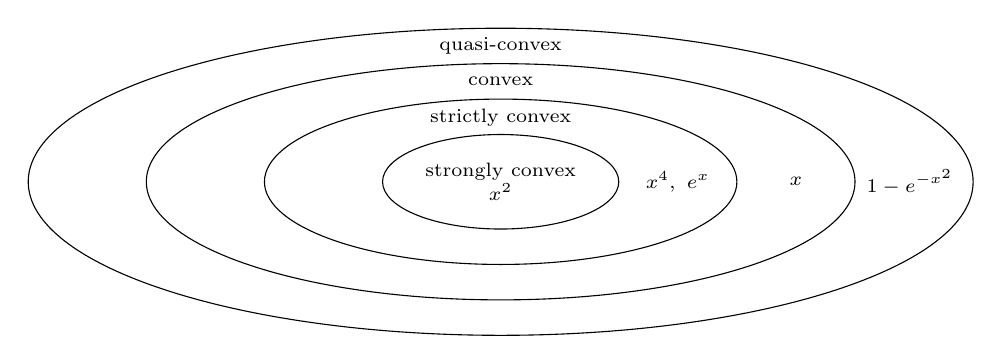
\begin{tikzpicture}[font=\small, lab/.style={font=\scriptsize, inner sep=1pt}]
  \draw (0,0) ellipse (6.0 and 1.95);
  \draw (0,0) ellipse (4.5 and 1.5);
  \draw (0,0) ellipse (3.0 and 1.05);
  \draw (0,0) ellipse (1.5 and 0.6);
  \node[lab] at (0,1.72) {quasi-convex};
  \node[lab] at (0,1.27) {convex};
  \node[lab] at (0,0.82) {strictly convex};
  \node[lab, align=center] at (0,0) {strongly convex\\[1pt]$x^2$};
  \node[lab] at (2.25,0) {$x^4,\ e^x$};
  \node[lab] at (3.75,0) {$x$};
  \node[lab] at (5.2,0) {$1 - e^{-x^2}$};
\end{tikzpicture}
